
\subsection{Radio Transceiver}
For the radio transceiver of WHCS the chip that we decided to use is Nordic
Semiconductor{}'s NRF24L01+. This chip meets all the requirements that we set
for our radio transceiver. The NRF is also a very popular chip that is easy to
find and rarely out of stock. This is a benefit to the manufacturability of
WHCS because NRFs are cheap and easy to buy in bulk. Alternatively we could
have chosen to use an XBee radio device which implements the zigbee 802.15.4
IEEE standard, however we did not see the need for this. XBee devices are also
more expensive than the NRF chips that we have decided to utilize.

\subsubsection{Operating Principles and Usability of NRF24L01+}
The NRF24L01+ is a radio transceiver that operates in the ISM (Industrial,
Scientific, and Medical) radio band. The range of channels for the NRF is
2.4GHz to 2.527 GHz, however because the designated ISM band that we are using
only ranges from 2.4GHz to 2.5GHz we will not be able to use all of the NRF{}'s
available channels. With the NRF we are capable of sending payloads with a
maximum size of 32 bytes per transmission from module to module. We will be
able to change the data length from 1 to 32 bytes in order to find the optimal
mix between reliability and speed. Every NRF chip has the ability to
simultaneously store 1 transmission address and 6 receiving addresses. The
first receiving address is utilized if the auto{}-acknowledgement feature is
enabled, so effectively there are 5 receiving addresses.  This capability gives
us flexibility for implementing our network because we make decisions such as
having a dedicated address to each node in the network as well as an address
for broadcasts of certain types. The addresses of the NRF are 5 bytes wide so
we will be able to have many NRF modules within the network. A very useful
feature of the NRF is the ability to enable auto{}-acknowledgement. When this
feature is activated the receipt of a transmission from one NRF to the other is
auto{}-acked without the need from any upper level software. This simplifies
the work necessary for creating our own network of NRF chips. We will be able
to confirm the receipt of data therefore increasing reliability.  This
auto{}-ack also allows the NRF to perform retries up to a given limit, so just
in case there is noise during the transmission the NRF will repeatedly try to
transmit again. The NRF also allows for low power mode and long range mode.
For WHCS we will be able to tweak whether or not to use long range mode or not
depending on the performance of the system within its environment.

The NRF requires 3.3v of electricity to operate so all parts of WHCS will
require a 3.3v line. The datasheet lists the current consumption while in
receive mode as 18mA. This will be the most common mode for the NRF chips
present in WHCS so they can be ready to receive commands at any time. The chip
receives commands from a microcontroller through SPI (Serial Peripheral
Interface). This is great because the NRF design philosophy fits perfectly with
our microcontroller based base station and control modules. Beside the standard
MOSI, MISO, and SCK for SPI, the NRF also has a csn pin for telling it to
receive commands, ce pin for telling to to transmit or receive at that moment,
and an interrupt pin for notifying the microcontroller of important situations.
The csn pin will allow the SPI bus to be shared with other components such as
the LCD being used for the base station. The interrupt wire pin can be
monitored in order to listen for data received, data sent, and data failed to
send notifications. In total the NRF will take up 6 pins whilst three of the
pins will be shareable with other SPI components.

\subsubsection{Driver Use Case}
The NRF chip that we have decided to use for communication in WHCS will need to
have a driver written for it. This will help keep the way we interface with the
NRF consistent and will provide clean code. All of the network code that we
write for the base station and the control modules will be relying on the
integrity of the NRF driver that we write.  The driver provides the foundation
and if it is not reliable then none of the code we write for our system will be
reliable. The focus for the development of the NRF driver is elegance. We want
everything the NRF driver offers to be simple yet accomplish everything
necessary. We have developed the use case diagram pictured in
\autoref{fig:nrf-usecase-diagram} as a guideline for the development of the NRF
driver. The NRF driver should provide the functionality included in the use
case diagram in an easy to use format.  These will be the most common uses of
the NRF.

\ucfgfx[scale=0.4]{fig:nrf-usecase-diagram}{a51-img001.png}{NRF Driver Use-case Diagram}

The core use of the NRF driver is transmitting and receiving payloads. Every
other use case is a supporting role for the final goal of transmission. The
basis of the driver will be reading and writing registers. Everything will
build off of this capability, especially reading and writing the payload for
transmission. Other use cases such as changing power mode, checking the status
of the chip, and changing from a transmitter to a receiver will be special
forms of writing to a register. Thus reading and writing to registers is a use
of the driver, however it will be abstracted in a way that provides ease of
use. A user of the NRF driver will spend most of the time setting addresses,
writing payloads, transmitting payloads, and analyzing interrupts. These use
cases need to be implemented perfectly to provide a strong foundation for the
networking of WHCS.

\subsubsection{Driver Class Diagram}
It was decided that the best design approach for implementing the NRF driver
was as a class in C++. We will be using Atmel ATMega microcontrollers in WHCS so C++
is supported as a development language. Using C++ allows us to create a class
that can leverage object oriented programming techniques such as encapsulation.
The class diagram for the driver is shown in \autoref{fig:nrf-class-diagram}.
Primitive functions such as ReadByte and WriteByte can be hidden from a user
while PowerUp will be exposed as a public function. Using C++ also gives us the
ability to use a constructor when using the WHCSNrf class, and in this
constructor we can assign the only thing varying between uses of the NRF, the
chip enable pin and the chip select not pin. Assigning the ce pin and the csn
pin are the first step of using the NRF driver. Any communication between the
microcontroller and the NRF will rely on the proper assignment of these pins.

%\begin{wrapfigure}{r}{0.5\textwidth}
%  \begin{center}
%      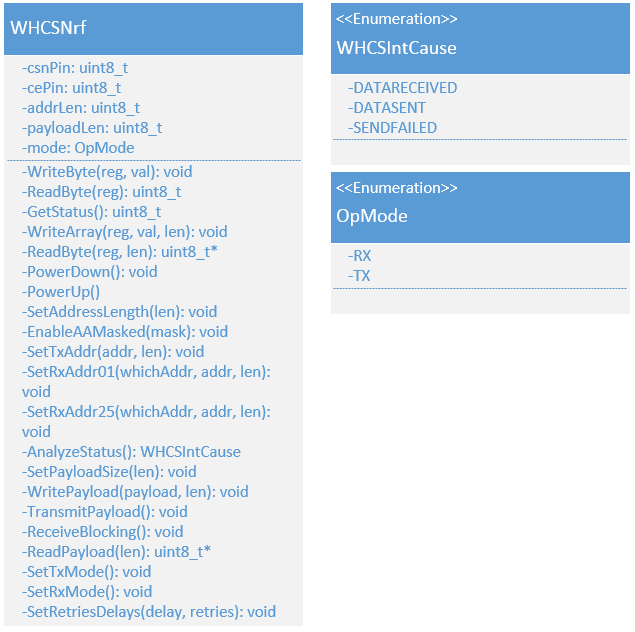
\includegraphics[width=0.48\textwidth]{a51-img002.png}
%  \end{center}
%  \caption{NRF Class Diagram}
%  \label{fig:nrf-class-diagram}
%\end{wrapfigure}
\ucfgfx[scale=0.5]{fig:nrf-class-diagram}{a51-img002.png}{NRF Class Diagram}

Usage of the NRF driver will involve first constructing the class by telling
the microcontroller which pins the NRF is connected to. Then the user will be
doing everything necessary to customize the way that data is transmitted and
received. The driver exposes the common settings in an easy to access manner.
Enabling things such as auto{}-acknowledgement and the number of retries for
the transceiver can be done with the call of a function with simple parameters.
Setting the address for receiving and transmitting data can be done in one line
of code. The SetTxAddr function will be one of the most utilized function for
an NRF involved in a network constantly sending payloads to other chips. A
typical use will involve powering up the NRF with the PowerUp call, setting the
transmission address, writing a payload, and then transmitting a payload. With
this driver, the user does not need to know the registers involved with the
NRF. The hardware interactions with the chip are all abstracted away.

\subsubsection{Network Library}
\label{sec:network-library}
\todo{3 pages}

In order for WHCS to be networked, a set of networking functions will have to
be constructed on top of the radio driver to form a network library or
\textbf{NetLib}. Abstraction of the raw driver will allow for the concept of a
\textbf{node} to be created. The network will consist of a set of nodes capable
of direct communication and reception of \textbf{logical packets}. These
packets will contain metadata describing their purpose and the data that they
contain. By dividing up the required network features of WHCS in to packets, we
will have a library of datagrams. These datagrams no longer have to worry about
low-level details such as when to transmit -- they merely have to worry about
who they are sending to and receiving from.

Similar to network protocols today, WHCS will implement a lightweight protocol
stack similar to the OSI model. The physical layer is handled by the NRF chip
itself, the logical link layer by the NRF driver, and all other layers by the
NetLib. In WHCS's case, our version of an ``Internet Protocol'' would be to
assign each node with unique ID that can be targeted by other nodes for sending
and receiving data. In terms of the transport layer, our application would be
similar to User Datagram Protocol, which is ``best effort'' in terms of
reliability. We plan on adding additional code and sequencing to allow for this
unreliable medium to withstand lost packets. The NRF already provides the
ability to retransmit on a non-acked frame, but this will just fail after a
certain amount of attempts. This would handle transient errors, but not a
complete loss of connectivity, which would occur if the base station lost
power.

In order to keep the network topology simple, we opt to have a simple module to
base network. This means modules will talk directly to the base station and to
no other modules. This is a simplification based on the underlying radio's
range and our project requirements. We do not need a complicated mesh network
as all of the nodes will be within range of the base station during their
lifetime. For larger or noisier households this architecture would break down,
but for the purposes of an initial design, this configuration will do the job.
Additionally, the network topology is not fixed in hardware - it is merely
additional code that needs to be written and implemented in to the overall
design. More research could be done along the direction of a full mesh network,
but only if necessary for good performance. The direct benefit of this simple
architecture is that is easy to test and easy to program. The logic will only
expect transactions to occur between two nodes. That fact will drive the
construction of a specific and optimized network communication protocol that
doesn't waste unnecessary bytes during transmission. The lower the byte count
for each transmission, the more likely the packet will reach the destination in
tact.

\paragraph{Modes of operation}
Before diving in to the specific functions required for implementing a robust
NetLib, we will discuss the high-level modality of the library. The state of a
network link can be broken in to the following modes:

\begin{itemize}
  \item Joining
  \item Communicating
  \item Idling
  \item Leaving
\end{itemize}

The network library will be in the \textbf{joining} mode when it is first
powered on or in the event of a disassociation. The node will attempt to join
on to a local network of nodes through a master node that is defined at the
initial hardware configuration of the network. The joining process will have
its own state machine describing the required processes for association on the
WHCS network. The \textbf{communicating} mode will be active if the node is
joined to a network and if there are data to be sent or received. Otherwise the
node will be in the \textbf{idling} state, which will include a reduction in
power consumption. If for some reason the network needs to be reconfigured
dynamically, the base station or a control module can begin the
\textbf{leaving} mode. This will free any resources present for maintaining
state on the active network join and prevent the leaving node from
communicating on the network. A graphical overview of the NetLib modes and the
transitions between modes is shown in \autoref{fig:netlib-state-overview}.

\ucfgfx[scale=0.75]{fig:netlib-state-overview}{netlib-state-overview}{the overall state machine for the network library}

\paragraph{Join mode detail}
The join mode will be fired when a new node wants to associate to an existing
WHCS network as maintained by a base station. The base station will be the
arbiter of all communication for the WHCS network and as such will also handle
initial join requests. It is the node's responsibility to know and maintain any
necessary access tokens for a join request along with the required channel of
the network. Having the required channel is required for the sender and
receiver to communicate. An optional (as per the setup configuration) will be
communicated during a join request. The base station will validate the joining
node and grant or deny access to the WHCS network. This process is necessary to
provide some assurance and tracking for the active nodes on the network.

\missingfigure{Join mode state machine}

\paragraph{Communicate mode detail}
Once a node has been successfully joined to the WHCS network, it will be able
to communicate directly with the base station as its network gateway. All
communication will flow through this node, which will process the data, and if
required, generate a response. This response may be directed back at the
transmitting node, such as an acknowledgement of the packet. Packets of control
modules have the ability to change state in the base station through the use of
``update packets.'' These packets will provide some periodic or event
information about the transmitting node. This could include arbitrary data an
is parsed based off of the node type. For example, a temperature node will have
a specific data format that the base station will know how to unmarshal and
store.

The overall flow of the communicate mode will be to pump out packets to be
sent, wait for any responses, and generate any actions as required by the
packets. This loop will be performed by any node with a radio. The base station
is the only special case as it has to receive from multiple nodes
simultaneously.
\missingfigure{Communicate mode state machine}

\paragraph{Idle mode detail}
The idle mode is the simplest mode for the NetLib. This state is where the
library has no data to send or receive. During this mode, the underlying radio
is free to sleep in order to conserve power usage. Also interrupts would be
used to avoid polling the radio for new data, which would eat a lot of power.
When a new packet is received or one needs to be sent, the radio would be woken
up and enter in to the communication mode.
\missingfigure{Idle mode state machine}

\paragraph{Leaving mode detail}
The final mode of the network library is the leaving state. This is the state
where the node decided or is ordered to leave the network. It will disassociate
from the WHCS network thereby causing its state and all of the resources
associated with the join to be freed. Additional cleanup will be performed in
order to get the library ready for a new join request. Any outstanding packet
sends or received will be canceled harshly and any potential data will be lost.
A safer shutdown would assert that the radio must be in the idle mode. That way
no data will be lost to the leave transition.  \missingfigure{Leaving mode
state machine}

%\begin{table}[H]
%\centering
%\begin{tabular}{|l|l|l|l|}
%\hline
%\bfseries Command & \bfseries Response & \bfseries Description  & \bfseries Direction \\ \hline
%ASSOC & ASSOC\_RESP & NODE\_TYPE,   & Node to Base Station  \\ \hline
%DATA & N/A & DATA\_TYPE, DATA & Node to Base Station  \\ \hline
%REQ\_DATA & DATA & DATA\_TYPE, DATA\_PARAMS... & Base Station to Node  \\ \hline
%ACTION & ACTION\_RESP & ACTION\_TYPE, ACTION\_PARAMS... & Base Station to Node  \\ \hline
%\hline
%\end{tabular}
%\caption{FILL IT IN}
%\label{tab:netlib-cmd}
%\end{table}

\subsection{Microcontrollers}
For the proper operation of WHCS microcontrollers will need to be installed
into all of the control modules as well as the base station. This meant
research was needed to choose what the best microcontroller for each of the
modules was.  The base station is a bit more hefty than the control modules so
the design considerations are different for the two.  The first step was to
figure out what family of microcontrollers to use.

\subsubsection{Microcontroller Brand}
Choosing the microcontroller brand would set the path for all the development
that we do with the microcontroller. Every other choice would stem from this
decision so we wanted to make a smart choice. We weighed out the documentation,
support, ease of acquisition, ease of use, and community for the brands that we
considered. Our initial choice was Texas Instruments because of the use of the
MSP430 launchpad board in the UCF curriculum. The fact that using the MSP430
was required in EEL 4742 (Embedded Systems) meant that everyone was already at
least somewhat familiar with it.  The familiarity factor was a plus for the
MSP, and we all knew that T.I. has very good, albeit lengthy, documentation for
their chips. A quick look at digikey showed that MSP430 microcontroller chips
were well in stock so there would be no problem acquiring them if they were the
chip that we wanted to use. The thing that we were unsure about with using
Texas Instruments chips was the community surrounding the brand. For example if
we encountered a problem rewriting a fuse on the microcontroller would we be
able to find a forum of people who knew how to solve the problem, and things of
that nature.

While we researched Texas Instruments based microcontrollers we also researched
the Atmel brand. We knew Atmel is very popular especially because they produce
the chip used on the Arduino development boards. We checked how the Atmel chips
were documented by looking at the datasheet for the Atmega 88, and were pleased
with how well things were laid out.  Digikey had most of the common brands of
Atmel chips in stock so acquisition would be no problem. We didn{}'t feel the
need to consider any other brands because we felt that between the two choices
we looked into they could both suit our needs. Atmel offered chips and brand
support similar to that of Texas Instruments, so for whatever kind of chip we
required we could use Atmel or T.I. For us the choice came down to how
prominent the communities for the two brands are. Ultimately we decided that
the Atmel brand had a very pervasive community that was sure to aid us in our
utilization of any chips produced by the company. While the MSP430 was familiar
to all of us the Texas Instruments chips did not seem as broadly used across
the open source populus. So our final decision was to use the Atmel brand of
microcontrollers for WHCS.

\subsubsection{Base Station Microcontroller}
The base station is the center of operations for WHCS so it needs the most
computing power. It has the most data structures to take care of, the most
commands to process, and the longest compiled program. The microcontroller for
the base station also needs to be able to connect to the LCD screen, the radio
transceiver, and BlueTooth transceiver all at the same time. So taking all
these things into consideration for choosing the microcontroller was important.
We needed a large amount of pins to interface with all the peripherals,
especially because we knew we wanted a parallel interface LCD. A large amount
of flash memory was also a trait that we looked for since we knew the base
station would be doing a lot, thus making its program long. The first big
decision was whether to use an ARM based microcontroller for our base station
since it was the brains of the system. ARM microcontrollers have much higher
processing power, but also introduce complexity. Many ARM microcontrollers
don{}'t have on board flash memory so that is an added layer of design that is
needed to get the unit working. After considering the processing necessary in
the base station and the bandwidth of the network in WHCS we realized that an
ARM based microcontroller would not be necessary. There was not enough data to
be processed to warrant the use of an ARM microcontroller. Using an ARM unit
would introduce design complexity for a solution that could be attained through
easier means.

Eventually our research efforts landed us upon the Atmega series of Atmel
microcontrollers. These microcontrollers are often thought of as the flagship
Atmel chips in the DIY community and they did seem highly capable. The chips
were cheap, had plenty of pins, plenty of on{}-chip peripheral support such as
the UART, were easy to program, and were highly available. After browsing the
Atmega series of chips we narrowed down the chip that we would be using for the
base station to the three chips listed in \autoref{tab:atmega-chips}. The table
shows that the lowest maximum operating frequency between the three is 16 MHz
which is more than capable of powering the low bandwidth network of WHCS. 16
MHz is enough to handle communication, the LCD display and interrupt vectors,
so all the chips are viable options in that feature. The 8 KB of flash memory
was low compared to the 32 KB offered by the other two so we actually took that
chip out of the running when we considered that the base station would have a
large routine. When we were down to choosing between the Atmega328 and the
Atmega32A we realized that the Atmega32A was actually the only option between
the two chips that would work. The reason for this was the number of I/O pins.
We had picked the LCD, radio transceiver, and BlueTooth chip that we would be
using and the Atmega32A was the only chip with enough I/O pins to support all
the peripherals. Our final decision was to use the Atmega32A as the
microcontroller for the base station.

\begin{table}[H]
\centering
\begin{tabular}{|l|l|l|l|}
\hline
{\color{black} Atmega MCU} &
{\color{black} Flash Memory (KB)} &
{\color{black} Max I/O Pins} &
{\color{black} Max freq. (MHz)}\\\hline
{\color{black} Atmega88} &
{\color{black} 8} &
{\color{black} 23} &
{\color{black} 20}\\\hline
{\color{black} Atmega328} &
{\color{black} 32} &
{\color{black} 23} &
{\color{black} 20}\\\hline
{\color{black} Atmega32A} &
{\color{black} 32} &
{\color{black} 32} &
{\color{black} 16}\\\hline
\end{tabular}
\caption{comparison of ATMega chips}
\label{tab:atmega-chips}
\end{table}

After we had decided to use the Atmega32A as the microcontroller for the base
station there were still some things that needed researching to make it usable.
The main issue was disabling the JTAG interface on port C to make the pins
usable as general I/O. After researching the data sheet and the community
forums we found that to be able to use port C pins as GPIO the JTAG fuse must
be disabled. Otherwise setting these pins on port C to high or low will have no
effect.

\subsubsection{Control Module' Microcontrollers}
The control modules are the parts of WHCS that do the interacting with the
endpoint appliances. The microcontroller that we selected for the control
modules would have to have the pin count and processing capabilities necessary
to be able to interface with any of the appliances. This means that the
microcontroller would need to have gpio pins for activating relays for the
outlets and lights, and it would also need to be able to do analog to digital
conversion for sensors. The control modules also receive commands from the base
station and send status replies back, so the control module microcontroller
would have to have an SPI interface for utilizing the radio transceiver that we
chose for WHCS.

The list of constraints on the selection of the control modules{}'
microcontroller was not long. The control modules were not going to be as
demanding as the base station. We could choose a minimalistic chip for the
control modules, but we knew it would help with the design and development
process if we used a microcontroller similar to the one in the base station for
the control modules. This led us back to the ATmega series. Referring back to
\autoref{tab:atmega-chips} we see the three main ATmega series chips that we
researched. All the chips had the SPI interface necessary to communicate with
the radio transceiver. They all had enough pins to interface with the most
demanding control module, and the all had analog to digital conversion
capabilities. Any one of the three chips would have been able to satisfy the
needs of the control modules. The ATmega88 was the first chip out of the three
that was removed from consideration for the base station. This was because the
on{}-chip flash memory was quite low. We decided not to use it in the control
modules for the same reason. The ATmega328 is only slightly more expensive than
the ATmega328 but has 4 times the flash memory. The ATmega32A, while useful for
the base station, would have been overkill for the control modules.  The amount
of pins on the ATmega32A would have taken up too much room on the board.
Therefore we decided to use the ATmega328 for the control modules.

For the control module microcontroller we also put research into using an
ATtiny microcontroller. The ATtiny series of Atmel microcontrollers are meant
to be low power and low pin count. If we could use an eight pin or similarly
sized microcontroller for the control module boards then it would save space
and therefore money on the printed circuit board. One issue that turned us away
from the ATtiny series was the lack of SPI and UART hardware modules on the low
pin count chips. For the chips that had SPI and UART support the pin count was
upwards of 20. This meant that there would be no large savings in terms of pin
count from the ATmega328 to a viable ATtiny chip. Thus we saw no reason to use
an ATtiny chip for the control modules rather than an ATmega chip.

\subsubsection{Development Environment}
To begin utilizing the microcontrollers that we chose we had to decide upon a
development environment to use. We believed that having everyone in the group
use the same environment would allow for easier collaboration and shorten
development time. Research showed that there were two popular choices for
writing programs for Atmel chips, Atmel Studio and WinAVR. Each of these two
environments had pros and cons. \autoref{tab:compare-atmel} shows relevant comparisons
between the two environments that led to the decision of what to use. The first
thing that we considered when choosing a development environment was cost. We
knew that certain IDEs, such as Visual Studio, require a license in order to
use. We thought that since Atmel Studio was based off of Visual Studio that it
probably required a similar license.  After looking into this issue we found
that Atmel Studio is free and WinAVR is also free. Knowing both are free we
took under consideration that part of the group mainly uses Linux.
Unfortunately neither of these development environments are usable on linux so
we all agreed to use the Windows operating system to host whichever option we
chose. Our next consideration was which IDE worked best along with the
programmer that we decided to use for the microcontroller. We decided to use an
AVR Pocket Programmer which uses a program called AVRDude for programming Atmel
microcontrollers. The Atmel Studio development environment could be set up so
the Pocket Programmer could be activated with the press of a button. This
capability was a noticeable win over WinAVR which elongated the process. The
feature that made Atmel Studio the clear winner of the two was the fact that it
provided so much sample code. Things such as the utilizing the UART or the SPI
interface for certain chips were about three clicks away while in Atmel Studio.
While the two IDEs did have many similarities, we all agreed that Atmel Studio
was the best choice for developing for our Atmel microcontrollers.

\begin{table}[H]
\centering
\begin{tabular}{|l|l|l|}
\hline
 &
{\color{black} Atmel Studio} &
{\color{black} WinAVR}\\\hline
{\color{black} Free} &
{\color{black} Yes} &
{\color{black} Yes}\\\hline
{\color{black} Linux Compatible} &
{\color{black} No} &
{\color{black} No}\\\hline
{\color{black} Integrated Compiler} &
{\color{black} Yes (GNU)} &
{\color{black} Yes (GNU)}\\\hline
{\color{black} AVRDude Integration} &
{\color{black} Yes} &
{\color{black} No}\\\hline
{\color{black} Sample Projects} &
{\color{black} Yes} &
{\color{black} No}\\\hline
\end{tabular}
\caption{Comparison of Atmel Studio and WinAVR}
\label{tab:compare-atmel}
\end{table}

\subsubsection{Microcontroller Additions}
To ensure that the microcontrollers we use on the base station and the control
modules are operating at their full capabilities we will be adding external
crystals to their circuits. The external crystals will boost the
microcontrollers operating frequency from their factory ratings of 1 MHz to the
native frequency of the crystal.  Because the lowest max operating frequency
for the microcontrollers we chose is 16 MHz this is the frequency we looked for
when choosing a crystal to use for the microcontrollers. We have decided to use
the NDK NX5032GA{}-16.000000MHZ{}-LN{}-CD{}-1 as the crystal for our
microcontrollers. This microcontroller has a 16 MHz operating frequency and has
the simple two connection design. For adding the crystal to our microcontroller
we will be using the circuit pictured in \autoref{fig:mcu-crystal}. The crystal
connects to the XTAL pins on the microcontroller and the microcontroller gets
its driving wave from the crystal. As the diagram shows there are two
capacitors that must be utilized to get the circuit working. These capacitors
are $C_{1}$ and $C_{2}$ and there is an equation for
choosing their value.

\ucfgfx[width=6.006cm,height=7.038cm]{fig:mcu-crystal}{a62expected5pages-img001.png}{Microcontroller Crystal Schematic}

The equation is for choosing the values for $C_{1}$ and
$C_{2}$ is shown in \autoref{eqn:req-cap} where
$C_{stray}$ is dependent on board layout and is approximately 2-5 pF
and $C_{L}$ is a property of the crystal. For our calculations we
used $C_{stray}$ = 3pF. $C_{1}$ also is equal to
$C_{2}$ so this simplifies the calculations. The value of
$C_{L}$ for the crystal we listed is shown as 8pF in the datasheet.
Using the given equation we found that the best value for the capacitors
$C_{1}$ and $C_{2}$ necessary in the crystal circuit was
10pF.

\begin{equation}
  C_{L} = (C_1 * C_2) / (C_1+C_2) + C_{stray}
\label{eqn:req-cap}
\end{equation}

To make the external crystals work with the microcontrollers, certain fuses
must be set through a programmer connected to the microcontroller. The
datasheets for the microcontrollers have a fuse list that can be used to make
the proper alterations for incorporating an external crystal into the design.
There is also a free online fuse calculator tool for AVR microcontrollers at
\url{http://www.engbedded.com/fusecalc/} that can be used to quickly get the
necessary fuses that must be changed for any sort of microcontroller alteration
such as changing the operating frequency.

To get the microcontrollers running the code we right needs to be programmed
onto the chips flash memory. Atmega microcontrollers use SPI to transfer
programs to the chip. There are different programmers that can be used to
complete the task of uploading code to the microcontroller. We put research
into which programmer to use in order to be the most cost effective with our
design. The two programmers that our decision came down to are listed in
\autoref{tab:comparison-of-prog}. Atmel has a programmer called the AVRISP mkII. This
programmer is supported by the designers of the chips so it is sure to work
when ordered however it also comes with a large price tag compared to other
options. The online vendor SparkFun offers a product called AVR Pocket
Programmer for \$15 that accomplishes all that we need to get our programs onto
our microcontrollers. The programmer relies on an open source program called
AVRDUDE to get the hex file from the development computer to the chips flash
memory. The program is free and the pocket programmer is much cheaper than the
Atmel programmer which costs \$34 if ordered from the Atmel site. The AVR
Pocket Programmer was a clear winner when it came time to choose the programmer
for our microcontrollers.

\begin{table}[H]
\centering
\begin{tabular}{|l|l|l|l|}
\hline
{\color{black} Programmer} &
{\color{black} Supplier} &
{\color{black} Price} &
{\color{black} Atmel Studio Compatible}\\\hline
{\color{black} AVRISP mkII} &
{\color{black} Atmel} &
{\color{black} \$34} &
{\color{black} Yes}\\\hline
{\color{black} Pocket AVR Programmer} &
{\color{black} SparkFun} &
{\color{black} \$14.95} &
{\color{black} Yes}\\\hline
\end{tabular}
\caption{Comparison of Two Different AVR Programmers}
\label{tab:comparison-of-prog}
\end{table}

\subsection{BlueTooth Chip}
The BlueTooth device for WHCS will enable the base station to communicate with
the mobile phone controller. Our guidelines for choosing a BlueTooth device
included ease of use, reliability, size, cost, availability, and documentation.
There were a multitude of BlueTooth devices to choose from. Special attention
was paid to how well the BlueTooth device could connect to a microcontroller
UART. Two BlueTooth devices, the HC{}-05 and the RN{}-41, showed the most
promise. Our research of the two devices showed that they both had their
advantages and either one could be implemented in our design. After careful
consideration we chose to utilize the HC{}-05 in our design, however the
RN{}-41 could still replace the HC{}-05 if necessary.

An important factor for considering the BlueTooth devices was if the internal
settings of the BlueTooth devices could be changed and if possible how. Such
internal settings include things such as the device{}'s BlueTooth name, baud
rate, and passcode. These things need to be changed from their default settings
or else many BlueTooth devices would have similar names, and they would all
have default passcodes. We want to implement good security into WHCS so we need
to be able to change the default passcode for the BlueTooth device. Also the
baud rate is usually low in BlueTooth devices by default, which can be bumped
up depending on the microcontroller being used. A BlueTooth device that could
not be programmed easily was not an option.

\subsubsection{RN-41}
The RN{}-41 is a BlueTooth module designed by Microchip. This module is
designed to be an all inclusive solution for embedded BlueTooth. It is clear
that a lot of design went into this chip because it is very high quality and
the data sheet is very thorough. Along with the high quality of the module
comes the high cost. Of the two considered BlueTooth modules the RN{}-41 was
much more expensive with a price of \$21.74 from Microchip. The high price tag
makes it a less appealing option out of the BlueTooth devices because they are
effectively accomplishing the same thing. The module itself appears well
designed visually and it has dimensions of 25.8x13.2mm so it is not obtrusive
and could fit well onto a PCB. There are 24 pins on this device and the
datasheet gives the dimensions down to the pin spacing allowing for easy PCB
layout design. The RN{}-41 makes communicating with microcontroller UARTs easy
by simplifying RS{}-232 down to the Rx and Tx wires. This means the only
connections necessary for using the RN{}-41 with a microcontroller are power,
ground, Rx, and Tx. The microcontroller{}'s that we have decided to use include
Rx and Tx pins that hook up directly to the RN{}-41. From the
microcontroller{}'s point of view the BlueTooth device does not even exist. The
RN{}-41 acts as a transparent man{}-in{}-the middle and simply relays messages
from a BlueTooth device to the microcontroller and vice versa. This is perfect
for our design because the RN{}-41 could just be plug and play. With an
advertised 100 meter transmission range the RN{}-41 meets the requirements we
set for distance of BlueTooth reception.  According to the datasheet the
RN{}-41 has a maximum baud rate of 921K which means it goes above and beyond
the transmission rates necessary for communicating between the mobile device
and the base station.

The RN{}-41 has a manageable means of programming the internal settings. When
the RN{}-41 is on, sending {}``\$\$\$'' over the UART lines puts the chip into
command mode. From here there are a list of commands that can be passed in
order to inquire or manipulate the state of the module. There are advantages
and disadvantages to this approach. It is great that it is easy to program the
RN{}-41 just by passing certain data while it is wired normally, however in the
event that the sequence {}``\$\$\$'' was ever passed during operation it could
throw off the whole system. This is not a terrible thing but it is worthy of
consideration.

\subsubsection{HC-05}
\label{sec:bt-hc-05}
The HC{}-05 is a BlueTooth module that shares many similarities with the
RN{}-41. It is of comparable size to the RN{}-41 with dimensions of 27x13mm.
HC{}-05 modules are also commonly sold along with a breakout board with male
headers. This makes it an option to have the PCB include female headers and use
them for installing the HC{}-05. Our intention for the base station containing
the BlueTooth module is to have the PCB board hidden, so using female headers
for plugging in the HC{}-05 to the PCB is a viable option. The module is
advertised as a low power class 2 BlueTooth device with power consumption for
communication listed at 8 mA. This is lower power consumption than the RN{}-41.
The max signal range is not listed in the data sheet, however we have tested
this chip and have achieved a signal range of more than 50m which is more than
enough for what we desired in our BlueTooth chip. Just like the RN{}-41 the
HC{}-05 communicates to microcontrollers by simplifying RS{}-232 and only using
the Rx and Tx pin. The maximum supported baud rate is 460800 which will allow
for very fast data transfer and will exceed the needs of communication speeds
in our system.

The HC{}-05 comes with default settings similar to most BlueTooth modules. The
default baud rate is 9600 and the default passcode is 1234. In order to change
this the module must be accessed in AT mode. AT mode is entered by utilizing
pin 11 {}``key{}'' on the HC{}-05. When this pin is held high, the module
enters AT mode on startup and is ready to take commands. This means that
whenever we want to program the BlueTooth module we will need to use a
microcontroller with a UART connection to a terminal as well as a UART
connection to the HC{}-05. This will require the implementation of a software
Rx and Tx pin. This will only need to be done once because once the BlueTooth
module has been programmed it retains that configuration. The requirement of
holding the key pin high during startup of the module eliminates the danger of
entering the programming mode during normal operation.

For WHCS we have decided to use the HC{}-05 as our BlueTooth module instead of
the RN{}-41. \autoref{tab:bluetooth-compare} shows highlights of the features of each
BlueTooth module that led to the decision. The main factors deciding this were
the cheaper price of the HC{}-05 and the fact that they both accomplish the
same thing. The table shows clearly that the HC{}-05 is a much more affordable
option. The two chips were comparable in size, features, wiring, layout, and
usability however at the price of \$6.64 the HC{}-05 cost less than half of the
RN{}-41. The RN{}-41 is the second best choice and can serve as a fallback if
HC{}-05 chips went out of stock or an unforeseen circumstance occurred.

\begin{table}[H]
\begin{tabular}{|l|l|l|l|l|l|}
\hline
 &
{\bfseries Cost} &
{\bfseries Range (meters)} &
{\bfseries Breakout Option} &
{\bfseries Configurable} &
{\bfseries Size}\\\hline
{\color{black} RN{}-41} &
{\color{black} \$21.70} &
{\color{black} 100} &
{\color{black} No} &
{\color{black} Yes} &
{\color{black} 25.8x13.2mm}\\\hline
{\color{black} HC{}-05} &
{\color{black} \$6.64} &
{\color{black} 50+} &
{\color{black} Yes} &
{\color{black} Yes} &
{\color{black} 27x13mm}\\\hline
\end{tabular}
\caption{comparison of the BlueTooth chips}
\label{tab:bluetooth-compare}
\end{table}

\subsection{LCD}
\todo{whole section}
Being able to interface with WHCS like a normal wall thermostat is one of our
project goals. Having a centralized display that can quickly display the most
important information for homeowners would be step up from traditional ``dumb''
thermostats. With a simple LCD combined with a touchscreen, users would have a
way to control and query their home without having to find their phone.

To make this a reality, we have chosen the versatile, premade, and well
supported Adafruit 2.8" TFT LCD\footnotemark{} with a resistive touchscreen.
Internally, the display is driven by the feature-rich
\href{http://www.newhavendisplay.com/app_notes/ILI9341.pdf}{ILI9341 chipset}.
This chip is specifically created for a 240x320 pixel LCD with a focus on
small, power-conscious mobile devices. Another reason we chose to buy this from
Adafruit and not integrate the chip directly is due to the complexity of the
design. Also, with the abstracted product, there are
\href{https://github.com/adafruit/Adafruit_ILI9341/tree/master/examples}{plenty
of usage examples} and Adafruit's
\href{https://learn.adafruit.com/adafruit-2-dot-8-color-tft-touchscreen-breakout-v2}{excellent
technical documentation}. This combined with Adafruit's
\href{https://github.com/adafruit/Adafruit_ILI9341}{libraries}, assure
that integrating the LCD will be straight forward. The one issue with
this solution is with the ILI9341 driver code: it was written to target the
Arduino platform. Now, the Arduino platform is fairly close to bare AVR, minus
the remapped pin numbers and some support libraries, so porting Adafruit's
library would be a feasible solution. Our plan is to use the existing driver
along with the chip datasheet to create a library specific to our needs. That
way we get full control over the port placement and the experience of creating
an LCD driver.

\footnotetext{\url{https://www.adafruit.com/products/1770}}

\subsubsection{Capabilities}
\todo{1 page}
In terms of capabilities, we have summarized the main features of the LCD module in \autoref{tab:lcd-features}

\begin{table}[H]
\centering
\begin{tabular}{|l|l|}
\hline
\bfseries Specification & \bfseries Description \\ \hline
Resolution & 240x360 \\ \hline
Colors & 262K @ 18bits, 65K @ 16bits \\ \hline
Voltage Input & 3.3 - 5V \\ \hline
Weight & 40 grams \\ \hline
Dimensions (LCD itself) & 2.8" diagonal \\ \hline
MCU Interface & Multiple. See \autoref{sec:lcd-driver}\\ \hline
Touchscreen technology & Resistive (one finger)\\
\hline
\end{tabular}
\caption{a brief summary of the pertinent features of the LCD module}
\label{tab:lcd-features}
\end{table}

These features are more than sufficient for out application as most of the
drawing we will be doing will be non-realtime. Nearly all of the displayed
information will be text and UI element, which don't change often. For an
overview of our UI elements, see \autoref{sec:ui-lib}.

One of the beneficial features of the LCD is that it gives developers a choice
of which interface to use. The broken out interfaces are 4-bit SPI and 8-bit
parallel. For prototyping, we used the low pin count SPI interface, but for our
final design, we will be using the 8-bit interface to avoid having to wait for
lengthy SPI transfers. Also, our NRF radio will be using the SPI bus, which
should have priority over that channel. You may view a high level overview of
the LCD module in \autoref{fig:lcd-high-level}.

\ucfgfx[width=\textwidth]{fig:lcd-high-level}{lcd-high-level}{a high level outline of the LCD pin configuration and specifications}

Another feature of Adafruit's module is the resistive touchscreen present on top of the
LCD. With this, we don't just have to display information about WHCS, we can
receive commands as well. Using this simple interface, we plan on creating a
featureful UI library to communicate up-to-date information about the home
while allowing for user control. The specific interface for the touchscreen
requires 4 pins, 2 of which must be connected to the MCU's Analog to Digital
Converter. By reading the resistance of the touchscreen, we would be able to
calculate the position of a single finger.

Finally, one extra component on the LCD module is an SD card slot. We are free
to read and write directly to this card to store large images, such as logos
for display on the LCD. We plan on storing at least our logo, but we may also
store fancy UI badges such as arrows ($\leftarrow,\rightarrow$), X's
($\otimes$), checkboxes (
\makebox[0pt][l]{$\square$}\raisebox{.15ex}{\hspace{0.1em}$\checkmark$}), and
anything else we can think of.

\subsubsection{ILI9341 Driver}
\label{sec:lcd-driver}
\todo{2 page}

In order to perform the required operations for drawing pixels to the LCD, we
need a robust driver to manage the state of the ILI9341 chip. This driver will
have to implement primitives for choosing a position to draw and the ability to fill
pixels.

\paragraph{Choosing where to draw}
The ILI9341 works like many chips in which it has a command set for controlling
display parameters. One of these commands will set the window in which pixel
data is drawn. Before a batch drawing operation, a window is selected by
specifying the column and page addresses. These are set using the
\textbf{Column Address Set (0x2A)} and the \textbf{Page Address Set (0x2B)}
commands. From this point, the RAMWR command is send followed by \emph{N}
different 16-bit pixel colors. This scheme of setting the window and filling
the pixels is why the graphics transfers end up being so slow, which is
discussed more in \autoref{par:lcd-perf}.

\paragraph{LCD State Management}
Beyond just drawing pixels, the LCD module has a wide variety of bonus features
that could assist us in making a fully-featured interface. One of these is
vertical scrolling, which could enable us to cheaply draw familiar UI elements,
such as list views. The most intensive state management comes from the early
initialization of the LCD module straight from power on. This requires a long
incantation of LCD commands with equally archaic parameters in order to reach
the initialized zen. Luckily, there are multiple examples of slightly different
LCD initialization sequences online for reference. In terms of power
management, the LCD controller provides a command set to set the power mode.
Although, the base station will be on wall power, being able to dim the screen
and save energy would be a useful feature.

\paragraph{LCD Performance}
\label{par:lcd-perf}
Due to the real-time nature of microcontrollers, everything must be juggled as
quickly as possible in order to have a good responsive design. A user event
such as a touch event followed by a graphics redraw should never take prioirity
over more important operations, such as sending and receving from the radios.
This is a common theme
throughout real time environments, so much so that highly specialized Real Time
Operating Systems have been created to provide \emph{assurance} that some
operation/action will complete within a specified amount of time. We don't have that luxury -- instead we must consider performance before we hit any performance walls.

The slowest part about managing the LCD are the synchronous transfer of
commands and pixel data between the MCU and the graphics controller. Each
ILI9341 command is 8-bits and before any pixel operation the CAS and PAS
commands need to be set. These commands have two 16-bit arguments.
For settting just one arbitrary pixel 104 bits would need to be sent. This is a
considerable overhead, so care must be taken to perform pixel operations in
batch. Obviously, an algorithm that generates random pixels on the screen would have very
low performance.

One other hit to potential performance is the lack of double buffering. The LCD
chip only has enough RAM for one set of graphics memory, which means active
drawing occurs on the viewing surface. In modern day graphics pipelines, double
buffering and even \emph{triple} buffering are common place as they eliminate
tearing and free the developer from having to clear the screen. On modern day
graphics cards, clearing the screen is an extremely cheap operation -- on the
ILI9341, it's just as expensive as every other drawing operation.

\missingfigure{class diagram}

\subsubsection{Touchscreen Driver}
\todo{1 page}
The touchscreen will need code dedicated to polling the X+, X-, Y+, and Y- pins
of the LCD. These will give voltage readings that can be used to calculate the
position of a single touch. They can be read by using the built-in ATMega ADC.
Due to their not being a dedicated touch controller,
interrupts cannot be used to sense sharp changes. This will add to the
processing time of the microcontroller's main loop as it will constantly have
to perform ADC operations and comparisons.

\missingfigure{diagram showing the touchscreen coordinates}

\subsubsection{Graphics Driver}
Unlike the previous ILI9341 driver, our graphics driver will be in charge of
taking the low-level primitives exported by the LCD driver and using them to
draw useful screen elements. These include text, lines, rectangles, circles,
and images. The driver will essentially contain a set of routines for drawing
these objects given a set of parameters such as length/width for rectangles,
radius and position for circles, and bitmap lookup-tables for the text. These
functions and more are already created by Adafruit, but for the experience and
control of designing the graphics routines, we choose to implement our own.

Due to the unique hardware and software constraints (i.e limited clock speed
and memory), we must take care to not exceed the capabilities of the hardware.
This means floating point operations, which may be required for shapes such as
a circle must be optimized or not used at all. A quick optimization for
floating point operations would be to use a $sin()$ lookup table and only
integer multiplications. These performance issues will be addressed as needed
and only if necessary. By avoiding unnecessary optimizations, we will save
valuable time for building out the library.

\paragraph{Algorithms Necessary}
The functionality of graphics driver depends on some core algorithms for
efficiently creating meaningful screen objects. One of these core algorithms is
\href{https://en.wikipedia.org/wiki/Bresenham\%27s_line_algorithm}{Bresenham's
line algorithm}. This algorithm needs to be efficiently implemented as it will
be the base for nearly every derived graphics operation. For example, a
transparent rectangle has four sides which results in four calls to this line
drawing function.

If there were any need for UI elements to be at different depths, then each UI
element would have to have its

\paragraph{Character Lookup Table}
In order to convey useful information, we will need to display text to the
user. This text will be stored in an efficient lookup table for quick drawing
operations similar. On a limited embedded
system like this, there is a limited amount of time that can be dedicated for
font rendering. To save on time, we will use an existing font available online.
Adafruit also bundles a font in with their graphics library that is implemented
as a function instead of a block of memory.

\subsubsection{UI Library}
\label{sec:ui-lib}
\todo{2 page}

\paragraph{ButtonView}
\paragraph{TextView}
Properties: length (uint16_t), width (uint16_t), depth (uint8_t), text (16
bytes),
\paragraph{ListView}

%\begin{itemize}
%\item line drawing algorithms
%\item wow
%\end{itemize}

\subsection{Android Application} For most WHCS users the mobile application
will be the only physical interaction they have with the application. When we
set out for development we wanted to make an easy to use application that would
attract users to stick with our system.  Operability and usability were
emphasized in our design process. We wanted an appealing U.I. without
complexity, after all we are targeting a simple solution to home automation.

\subsubsection{Development Environment} Android is the mobile operating system
that we chose to utilize for our BlueTooth enabled phone. The Android operating
system is accessed through the Java language, which is a staple in the UCF
curriculum therefore everyone in our group is versed in it. Developing on
Android is also a free endeavour where as developing on an iPhone requires
enrolling in the Apple Developer Program. These programs actually cost a good
amount of money that is unnecessary to spend. The Windows Phone platform is
another option for the BlueTooth enabled phone, but they are very unpopular so
we chose not to target this platform. With our target narrowed down to the
Android operating system, we had to research what the best environment for
developing our application would be. There were three options that we
considered for managing the Android project each with their own perks: command
line tools, Eclipse, and Android Studio.

The first development environment we considered for our Android project was
creating our own project structure and using command line build tools. There
are also debug tools available on the command line for Android projects. These
tools would be necessary in order to do our testing on Android Virtual Machines
running on our computers. This approach favors people who are command line or
terminal oriented. Linux is popular within our group and the ability to do
things from the terminal is appealing so this approach seemed like a good one.
We realized that with the design we had in mind for our project, it would
become quite large and it might be difficult to handle without a dedicated IDE
(Interactive Development Environment). This led us to looking into using
Eclipse for developing our Android application. Eclipse seemed like a natural
choice because it is what is recommended for using in the Java oriented UCF
programming classes.  The Android SDK provides an add{}-on for Eclipse that
makes it a viable Android development environment. We were able to get this
running and create sample Android applications. Inside of Eclipse the project
structure for Android applications is laid out nicely. The debug tools are all
organized at the top of the screen resulting in an easier development
experience than debugging from the command line. The problem with using Eclipse
as our IDE is that Eclipse is notorious for being slow and unwieldy.

\color{black} Recently Google released a development environment named Android
Studio that is made specifically for developing Android Applications. No one in
our group had any prior experience using this IDE, however we realized that due
to it being tailored specifically for Android it was probably better than
anything else. This turned out to be correct, because it was much easier for us
to create an Android project and navigate our code from within this IDE. We
also decided to use Android Studio because it has built in Git support for
source control. This meant that as we were
writing our code we could easily submit our changes to a remote Git repository.

\subsubsection{Use Case Diagram} The central use cases for WHCS are toggling
the state of certain devices within the home and monitoring certain states.
For example a user of WHCS will spend most of the time turning on lights,
checking whether a light is on, or checking the temperature reading of a
certain sensor. There are certain other use cases that are necessary in order
for WHCS to be a functioning application, as well as to make it have a robust
feel. Features like speech activation and creating endpoint groups are
usability features that are not necessary in order to accomplish the central
goals of WHCS.  Connecting to the base station the first time you use the
application is a necessary use case that must be incorporated into the
application. \autoref{fig:android-usecase} shows the use case diagram for the
WHCS application.

The design for the WHCS application involves making sure that performing the
common use cases such as checking status and toggling endpoints are very fast.
The user should be able to perform these tasks without having any knowledge of
how the application works. Speech recognition will be a supporting feature so
it does not need to be a central focus like the area that will visualize the
control modules. When the user wants to perform speech activation it will
involve pressing a button to prompt the speech recognizer, and then giving a
command to the WHCS. In order to make the speech activation feature more
promising, the user will have the ability to rename endpoints for activation.
Creating endpoint groups will be a feature that is not used frequently but adds
a lot of value to the application. Users will only have to create an endpoint
group once for it to last in the application. Creating an endpoint group will
be a simple task involving assigning a group number to endpoints. That number
will be the endpoint group, then that endpoint groups state can be toggled.

\ucfgfx[scale=0.45]{fig:android-usecase}{a55-img002.png}{Android App Use-case diagram}

\subsubsection{Speech Recognition} The Android application for WHCS will offer
speech activation capabilities. These will be on top of GUI activation
capabilities. The speech activation sequence begins with the press of a button
to start the speech recognition. The user will be prompted with a microphone
and can then give his command. The commands will be formatted like {}``light
one on.'' When the user gives commands using the speech method, a notification
will be given indicating the success of interpreting the speech into a known
command. If the user{}'s speech does not match a known command, the speech will
be shown back to the user to show what went wrong. We are predicting that the
most frequent cause of this will be the Android phone mishearing the user. In
the event that the speech matches a command, the application will display the
command to the user and then perform it. The following flow chart in
\autoref{fig:android-speech} displays the sequence of events happening when a
user performs speech activation.

\ucfgfx[scale=0.4]{fig:android-speech}{a55-img003.png}{Android app speech activation
chart}

The goal of the speech activation feature is to be easy to use. In order to
promote the usage of this feature we will add the ability for users to rename
the endpoints that the speech commands will target. For example the user could
change {}``light 1'' into {}``living room light.'' This way the user could say
{}``living room light on{}'' to the application in order to turn on the living
room light. To do this data structures will need to be stored in the
application which hold the preferred name of each type of endpoint. Endpoints
can be distinguished by the type they are, their individual identifier number
and their preferred name. The preferred name should be stored when the
application is closed so a permanent source of storage is needed to do this.
The file system can be used or possibly a SQLite database.

In the code for our application we will be using the Android speech recognition
API (Application Program Interface).  Android has a speech recognition service
that can be started by requesting it within an application. We will request
this service to be run by using an Android construct called an intent,
specifically the recognizer intent. Once the request the service to be run it
gives us the text that it produced from listening to the user{}'s speech. The
code that performs this process ends up bloating up the application so we
sought to develop a wrapper class in order to perform the request for the
speech service and simply hand back the text. However because of the Android
design philosophy, creating a wrapper class to start the speech recognition
service was not easy enough to make it a worthwhile endeavour. Thus we
concluded the best approach is to keep the calls to the Android speech
recognition API within the class we use for our main activity.

\subsubsection{BlueTooth Software Design} BlueTooth will be the technology that
allows WHCS users to interact with the base station from the mobile phone. This
means that proper functioning BlueTooth software must be written to ensure that
users can interact with WHCS. From the user{}'s standpoint the only knowledge
of BlueTooth required will be the ability to perform an initial connection to
the base station. Once a user has connected to the base station once through
the WHCS app we will be able to cache the base station device and allow for
automatic reconnection every time the application is launched. This is an
important abstraction for the user because the user should not have to spend
time handling BlueTooth connections every time they open the application.
\autoref{fig:android-bluetooth-start} shows what the BlueTooth software will be
doing whenever the user opens the Android application.

\ucfgfx[scale=0.4]{fig:android-bluetooth-start}{a55-img004.png}{Android BlueTooth Startup
Flowchart}

In \autoref{fig:android-bluetooth-start} we see that the first check that is
made is to ensure that BlueTooth is enabled. The Android operating system
requires applications to ask the user whether they want to activate BlueTooth
or not. It cannot just be turned on. If the WHCS application is opened and
BlueTooth is off we will prompt to the user to turn it on and if they refuse we
will exit the application. When it has confirmed that BlueTooth is on, the
application can check to see if it knows the base station device. If the base
station device is known then the application can skip asking the user what to
connect to and can perform the connection automatically. This is what should be
happening most of the time. If the base station is not stored in the
applications data then the application will have to prompt the user to connect
to a base station. When connecting to a device there are two possibilities for
connection, paired devices and non{}-paired devices. The application will first
show the user all devices that their phone has paired with previously, in case
the application somehow forgot the base station. If the base station does not
show up in the paired devices list, the user will be able to search for active
BlueTooth devices and select the base station. At the end of this start up
cycle the WHCS application will have an active BlueTooth connection with the
base station that can be used for full duplex communication.

Our application will be leveraging the API and design guideline for using
BlueTooth from Android phones. The underlying driver for BlueTooth
communication utilizes sockets similar to network sockets in other languages.
Android offers a class named BluetoothDevice which contains all the address
information necessary for opening a socket. When our application scans for
devices or asks the user to pick an option from the list of paired devices this
will be to get the BluetoothDevice to open a socket from. Once we have obtained
that BluetoothDevice we can create a BluetoothSocket through one of its
methods. Once a BluetoothSocket has been opened through calling connect, an
input and output stream become available that allow us to send and receive raw
byte data. This is a primitive form of communication but it is also exactly
what we want. All data that we send or receive from the base station over
BlueTooth will be in the form of a byte array. This form of primitive data
transmission allows us to implement certain communication protocols between the
Android base station.

Once a BluetoothSocket has been opened on the Android device the application
can begin communicating with the base station. We will use a communication
protocol between the Android device to ensure the base station can properly
interact with the application. This protocol will allow the Android application
to give commands to the base station such as inquire about the state of the
control modules or to toggle state within the system. Whenever the Android
application wants to send a message to the base station the software will
create a packet with a certain structure. The packet will contain a byte for
letting the base station know that a command is being given, the command
itself, any variables for the command, and then a byte for finishing the
command. The base station will receive one byte at a time due to the serial
nature of BlueTooth communication but it will be able to parse the packets it
receives in order to figure out what action the application is trying to
perform. \autoref{fig:android-comm} shows a visual representation of the
communication between the aplication and the base station.

\ucfgfx[scale=0.4]{fig:android-comm}{a55-img005.png}{Visual of Communication Between
Android Device and Base Station}

\subsubsection{GUI Philosophy} Our goal for the development of the user
interface was to make something simple that users could navigate quickly and
efficiently. There is no need for the UI to be deep or hold the user{}'s
attention. The only purpose of the GUI is to provide intuitive visuals for
interacting with WHCS. When we developed the GUI we wanted to minimize the time
it took for the user to open the application and make a change within the
system. For example the user should be able to open the application and turn a
light on or off in the shortest time possible. This means opening up to a
screen that lists all possible end points in the system that can be targeted by
a command. The top right layout in \autoref{fig:android-gui} shows the view
that would list all of the accessible control modules in the system.

\ucfgfx[scale=0.55]{fig:android-gui}{a55-img006.png}{Android GUI Layout}

As shown in \autoref{fig:android-gui} there are layouts that provide support
around the main list layout. The first two layouts in the upper left and upper
middle are the what the user would see when the base station is not known to
the application yet. The user would need to select the base station from a list
of paired devices or perform a BlueTooth scan for active devices. Once the user
has selected a base station then the base station can be saved in the
application and the user should be able to avoid seeing these screens again.
The user would be viewing the main list layout at this point. From the main
list layout the user can navigate to the individual control module viewer. This
will be achievable by clicking on the name of a control module or by clicking
the edit button. The individual detail viewer will allow the user to toggle the
state of the control module, change the speech recognition name of the control
module, and assign the control module to a group. The detail viewer will also
list the current state of the control module.

In Android different aspects of a GUI can be created in two different ways,
fragments and activities. Typically fragments are used when two different
screens serve very similar purposes or are trying to accomplish a shared goal.
Fragments are typically used when exchanges are meant to be done very fast
between screens. In the case of our application we will be using separate
activities for each of the screens. This is a logical approach because the
layouts in our application are independent of one another. The main list layout
will serve as the root activity and any other screen will be an activity that
is placed upon it. For example when the application opens up the first time it
will try to open the list activity but will notice that it is not connected to
the base station. This will cause the paired devices activity to stack on top
of the list activity. When the base station is selected the paired devices
activity can return the result of the selection to the list activity and the
list activity can function normally. When the detail viewer activity is called
it stacks on top of the list activity and when the user is done with it, it
will be removed off of the stack.

To make our list activity look clean and function effectively we will create a
custom adapter. In Android, adapters are the classes that allow objects to be
transformed into data that a listview can turn into list items to be displayed
to the user. The name of the adapter will be cmAdapter. The cmAdapter that we
create will have an array of control modules as one of its fields, as well as a
function named getRow that it inherits from its base class Adapter. The
cmAdapter will know how to get the data from a control module object necessary
to populate the main list. The main list activity will constantly call the
getRow method that will be present in our adapter to fill the list. This
creates a nice object oriented design for listing all of our control modules.
If we want to display different data for control modules, we can simply alter
the getRow method that is implemented in cmAdapter.
\autoref{fig:android-class-diagram} shows the class diagram for the cmAdapter.
The class is simple but provides important functionality for the Android
application.

\ucfgfx[scale=0.4]{fig:android-class-diagram}{a55-img007.png}{\texttt{cmAdapter} Class
Diagram}

\subsubsection{BlueTooth Listener Class} When the WHCS application is
communicating with the base station it is easy for the base station to be
interrupted and start parsing communication using the UART interrupt vectors on
the microcontroller. We want our application to possess the same event driven
capability so we created the BlueToothListener class. This class handles
listening for any incoming BlueTooth communication aimed at the phone. The
class must be initialized by telling it what BlueTooth device it should be
listening for. Once this happens it can create a thread and constantly check to
see if the BluetoothSocket{}'s input stream contains any data from the target
device. If the inputstream contains data then we know that the target device
has transmitted to the application. The BlueToothListener class raises an event
whenever receipt of data has been confirmed. This allows the application to
conform to event{}-driven Android philosophy. We can design around the
BlueToothListener class and subscribe to the event it raises whenever data has
been received. This is one of the core classes for communicating with the base
station. \autoref{fig:bluetooth-listener} shows the class diagram for the
BlueToothListener class as well as the classes associated with it.

\ucfgfx[scale=0.45]{fig:bluetooth-listener}{a55-img008.png}{\texttt{BlueToothListener}
Class Along With Supporting Data Structures}

The BlueToothListener allows the application to directly hook up a parser for
the incoming data. We can create a custom class that parses incoming byte
arrays and transforms them into an understandable format for the application.
This class would implement the interface for handling the data received event
and could dictate what happens when certain data sequences are received. For
example when the application asks the base station what control modules are
currently known and active the base station would respond raising the data
received event. The parser would begin working on the data received because it
would have been subscribed to the event. The parser would realize that the data
received is an indication of the state of the system and would have a case for
handling what to do when this type of information is received. This would be
how the communication protocol for receipt is implemented on the Android
application.

\subsection{Power Hardware}
\label{sec:power-hw}

Throughout this section we will be discussing all that deals with the power.
For reasons that will be discussed in greater detail in
\autoref{sec:power-through} we decided that each control module and the base
station would have a power board that would be separate from the PCB of the
control modules and base station.  The reason for each power board is to
convert 120VAC to DC lines of 3.3V 5V and 12V. We will also need to be able to
switch on and off 120VAC for the outlet and light switching control modules as
well switch on and off the 12V used to operate the strike.

\subsubsection{Design Summary}
\todo{Joseph needs rewrite}

\subsubsection{DC-to-DC Converters vs. Linear Voltage Regulators}
In our control modules and base stations we are required to provide lines of
three different voltages 12V, 5V and 3.3V. This can be accomplished with a
voltage regulator or a DC to DC converter. Voltage regulators are variable
resistors that dissipate energy as heat to get the desired voltage levels. The
advantage of voltage regulators is that they are cheap. The issue is that they
are highly inefficient. Linear voltage regulators are good for low power
applications where not too much power will be wasted due to inefficiency.
Whereas DC to DC converters are more appropriate for large step downs in
voltage.

The basic tradeoff between the two technologies is cost vs efficiency. Dc to DC
converters are capable of achieving efficiency levels as high as 95\% but cost
close to \$10. The efficiency of linear voltage regulators depends on the
difference between the input and the output voltage. Yet the cost of a linear
voltage regulator is usually below \$2. Power wasted in a linear voltage
regulator can be determined by using \autoref{eqn:power-waste}.

\begin{equation}
P_{wasted} = (V_i - V_o) * i_l
\label{eqn:power-waste}
\end{equation}

Where $P_{wasted}$ is the power wasted, $V_i$ is the input voltage, $V_o$ the
output voltage, and $i_l$ the load current.

The basic question becomes how large of a stepdown are you expecting to have
from your regulators. In our design (mostly because of the backup battery) we
decided to have a step down from 34 volts down to 5V and/or 12V, as well as a
step down from 5V down to 3.3V. Based on these step down values it makes most
sense for us to use a DC to DC converter to step down 34V to 5V and/or 12V, and
to use a linear voltage regulator in order to step down from 5V to 3.3 volts.

\subsubsection{Backup Battery Configuration}
Each control module along with the base station in WHCS will be equipped with a
backup battery. In the case of power failure WHCS will still be able to carry
out the basic function of checking the state of the system. Actual operation of
some of the control modules will be impossible without the use of AC power. Yet
checking statuses such as temperature and the position of door locks will still
be fully operational. This is meant only to serve as a short term solution to
power failure.

Here we will consider different designs to make a backup battery. We{}'ll start
with the circuit that was actually selected to be used in our design. The
circuit below was made in Easy Circuit. The idea for the design came from the
following link

\ucfgfx[width=12cm]{fig:backup-bat-circuit}{a563expected2pagesBackBattery-img001.png}{chosen backup-battery configuration\protect\footnotemark}

\footnotetext{Design idea taken from \url{http://www.instructables.com/id/Simple-5v-battery-backup-circuit/}. Circuit remade.}

This design is simple. The circuit being open indicates when there is a power
failure, while a closed circuit signifies normal operation. The circuit shows
two sources, one (the one farthest to the left) that is of a higher voltage and
acts as the primary source and a secondary lower backup voltage source. Since
the secondary source is of lower voltage it will not discharge until the
voltage of the first source drops below a certain level. This is how tradeoff
occurs.  The secondary source has no potential until the first sources
potential drops below a certain level. In \autoref{fig:backup-bat-circuit} we see that
during normal operation (closed switch) that this design will recharge the
batteries, that is if the batteries are rechargeable. This feature can easily
be taken out by removing the diode and the resistor that feed into the
secondary battery.

In this design it is very important that the secondary source be of a lower
voltage than the primary source. If this is not the case the batteries will
discharge even when the primary source is functioning properly. Initially we
believed that this would be a handicap for our project and that a new design
would have to be used. Yet we realized that there was a way to ensure that the
primary voltage was higher than the secondary voltage. If we were to place the
backup battery before the DC to DC converter, and allow the DC to DC converter
to do a large portion of the voltage step down.  Say we had the the transformer
only transform down to 24VAC (roughly equivalent to 34 VDC) then had the DC to
DC converter bring the voltage down to 5VDC. Our primary voltage would be 34V
and our secondary backup source could be anything lower than 34V that is
accepted by the DC to DC converter.

Designing in such a fashion has it{}'s advantages and it{}'s disadvantages. The
benefit of placing this design right before the DC to DC converter is that no
matter what the voltage is coming into the converter (as long as it is within
the range or acceptable voltages for the converter) the output will always hold
the same voltage level. The main disadvantage is that the required voltage rage
needed by the voltage regulator may cause us to need higher voltage batteries
than we would have needed otherwise. Say for example we need a 5V line, the DC
to DC converter takes voltages from 9V{}-40V and converts it to 5V. For our
back up battery we are now required to use a 9V battery whereas in another
design we may have been able to get away with a 6V battery source.

Because of the high efficiency level of the DC to DC converters using a higher
voltage battery than may have been required is not a problem of wasting power
rather a problem of design cost. 9V batteries cost around \$6 for a pack of two
while AA batteries cost about \$14 for a pack of 24. The cost difference a 9V
battery and a 6V source with AA batteries is \$0.33. The 9V battery is more
expensive but it actually isn{}'t that much more expensive. The cost/volt of a
9V battery is better than that of the AA batteries.

The design above works because we have decided to use a DC to DC converter with
a decently sized voltage step down.If however this were not the case and the
primary and secondary designs were much closer in voltage levels than an
alternative design would have to be used. There are a few other design
possibilities that were explored.

Another design that was explored was to use a relay in order to drive the
switch. In \autoref{fig:backup-bat2} current flows from the primary source to
ground which activates the relay allowing the primary source to power the load.
If there were a power failure in the primary source the relay would switch to
circuit with the backup battery and thus the secondary source would take over.
The main issue with this circuit is that it requires a line that goes directly
to ground, thus wasting energy. The effect of this can be lessened by choosing
a large resistor value. Yet in the end we decided to go with the first design
because it provides the simplest solution.

\ucfgfx[scale=0.5]{fig:backup-bat2}{a563expected2pagesBackBattery-img002.png}{another backup battery configuration\protect\footnotemark}

\footnotetext{This schematic was constructed using Easy Circuit, and the idea for the
schematic came from a
\href{http://electronics.stackexchange.com/questions/96632/12v-battery-backup-supply-for-gprs-tracker}{StackExchange
post}.}

\subsubsection{Transformer Choice}

\subsubsection{Power Consumption}

\subsubsection{Isolation}

\subsubsection{Power Through Hole Board}
\label{sec:power-through}
Sending in PCB{}'s to be built can be expensive. Also the size of the boards
have a large impact on the cost. Due to the fact that components found in power
designs are large and will therefore be costly to place on a PCB we decided to
self build a separate board for power. Not only is this an advantage because it
is cheaper but it allows us keep high voltage AC isolated from the DC used for
our control modules and the base station. Additionally each of our power boards
are slightly different from one another so making our own boards will make it
easy to customize each board for their specific needs.

After deciding that we needed a separate power board we had to decide how to
build the board. The three candidates were: perf boards, vero boards, and
etched PCB boards. Out of the three the team decided that an etched PCB would
be the cleanest and would look more professional than an a perfboard or
stripboard. Next we decided that a through hole board would be superior to a
surface mounted board; mostly due to the fact that power boards can contain
heavy components (for example transformers) and through hole boards are more
mechanically sound than surface mounted boards.

In order to build our board we will be using Rogers RO4003. The primary reason
we decided to use Rogers was because they provide free samples for learning
purposes through their University Sample Orders Program. Since this is in fact
a non commercial academic project we were able to order a sufficient amount of
laminate material to complete our project.  RO4003 is a double sided laminate
typically used for high frequency applications. Building this board from
scratch will give added experience to the members of the group, which is the
ultimate goal of this project.

\subsubsection{Schematic}

\subsection{Base Station}
The heart of WHCS resides with the base station (BS). When users think of WHCS, they
will think of the base station as it is the most visible part of the system.
The base station is responsible for managing, collecting, and displaying
information from all of the control modules. If the BS were to fail, WHCS
would cease to function.

When a new control module is introduced in to the system, it must first pair
with the BS, which will authenticate it on to the network. Once it joins, the
control module can be abstracted as an ``API'' meaning, the specific hardware
details do not have to be considered. This abstraction will be excellent in
keeping the system clean from one-off cases and allow for a Domain Specific API
to be formed.

\subsubsection{Software Flow}
The main software flow for the base station is the most complicated in WHCS. It
has to manage three separate devices simulatenously and be able to service each
one in a timely manner. The LCD, NRF radio, and Bluetooth module are all being
controlled and commanded by one ATMega32-A chip. There isn't much room for busy
waiting or any expensive operations as everything has to be running as fast as
possible. Given this, the BS is the least point of failure for the WHCS.

In \autoref{fig:base-station-flow}, we have constructed the general architecure
of the main loop for the BS, including some early initialization. Most of the
implementation details are left out as they are very specific to the final
drivers.

\ucfgfx[width=0.8\textwidth]{fig:base-station-flow}{base-station-flow}{the high level software flow for the base station}

The large amount of tasks that are required of the BS become clear when viewing
\autoref{fig:base-station-flow}.

The base station from reset would first load any saved settings from the
EEPROM (saved control modules, behavior settings, LCD settings, etc.), then it
would bring up all of the main modules (radio, LCD, BlueTooth, and UART). If
any of these initialization steps were to fail, the BS would indicate through
an LED or from a UART debug message. An initialization failure shouldn't be
handled as it's a critical failure of the system along with its assumptions. We
believe that by assuring that the initialization sequences for all modules is
well defined, we will be able to diagnose hardware issues quickly and without
strenuous debugging. One of the issues we found while prototyping is that it's
difficult to determine if the issue with module initialization is with the
wiring or code. Having a golden model for code that is know to work on our
target setup would allow us to have a good working state.

Each module has a unique sequence of ``commands'' with parameters that are
required to configure the device. The NRF radio has to have its power, channel,
payload length, and other parameters set before usage. Once these basic
options, any further configuration is done at run time. This would include
switching from listening to transmitting mode and enabling or disabling the
automatic acknowledgement feature. The built-in Atmel UART only needs to know
the baud rate at which data will be sent and received. There are also other
options relating to other bits used (parody, stop, etc.). In our case, we are
using the default 8 bit data, 1 stop bit, which is simple enough for our needs.
The LCD happens to have the most extensive initialization sequence due to
required screen configuration, gamma settings, pixel order and other more
archaic options.

Once all of the modules are brought up correctly, the BS would begin the main loop.
Radio events, BlueTooth events, and LCD state would all be processed as
required. For both the BlueTooth and radio, new packets would be checked for
and serviced as needed. From these packets, internal state would updated and any
response packets would be generated and sent. Internally, WHCS will have an
internal event queue with different event types. These events will be processed
and any responses will be generated, if any. These responses could include a
confirmation packet over the NRF radio, or a status update through BlueTooth.
The base station may also initialize actions despite not receiving events.
These could be triggered from timers firing.

In terms of the NRF radio, the module we have chosen exports an interrupt pin
which will fire on the reception of a new packet. This feature is great for the
WHCS architecture as the radio requires a significant amount of power
while actively receiving SPI commands and transmitting. By avoiding the polling
of the NRF, the main loops for both the control module and base station will
have more cycles to process more important and intensive tasks. Essentially,
the NRF will be kept in the listening mode at all times, waiting for a packet
from a control module to be received. This is in contrast to the control
modules which will try to avoid the transmitting and listening states to save
power. The power down mode is great for saving watts, but has very poor
performance for quickly responding to new packets.

The BlueTooth module won't require as much time to service as the other modules
due to the low data rate. It will connected directly to the hardware UART of
the base station, instead of the normal serial debugger. This will have to be
connected to some free GPIO ports and software serial will be used. This is
unfortunate as ``bit banging'' serial isn't efficient and will take up many
more cycles than just using the hardware UART. If needed, a packet over
BlueTooth could be sent asynchronously from the main loop due to the hardware
UART. If the micro loops fast enough, then it would be as if there was no delay
in transmission. Due to the real time nature of the NRF radio and LCD, WHCS
will take steps to avoid blocking too long on a single activity. Blocking too
much will lower the overall performance and responsiveness of the system. At
worst, touch events could be lost and packet buffers could overflow. Until the
system's code is ready, this worry cannot be confirmed, but an effort will be
made to profile the main loop's average time using hardware timers.

One of the most important parts of WHCS is its usage of timers. A global list
of timers will be constantly maintained and updated to schedule events
in the future, instead of having to handle them immediately. The granularity of
the timers will depend on the average execution time of the main loop along
with how many timers are processed at once. If the main loop is slow on
average, then timers will have to wait for extended periods to be serviced
(starvation). Depending on the criticality of the timer and the event
associated with it, there may need to be a mechanism for assigning a priority
for a timer. This will have to be determined during actual system programming
as it is heavily dependent on the task required.

All of the above tasks will be executing in the same way as single core CPU
would: in pseudo-parallel. The faster the whole system runs, the better the
appearance of everything executing at once.

\subsubsection{Control Module Abstraction}
For WHCS to function smoothly and scale well, a neat and abstracted interface
must be defined to accept \emph{any} type of control module. New control module
types should be easily added to the system without affecting older types and
there should be a set of generic data structures for managing and storing
information on modules. These structures must be carefully defined to wrap more
specific control module packets in all of the shared metadata. Think of it like
a hierarchy where all of the common attributes and actions shared by control
modules have packets that can be sent to any module. Whereas the more specific
packets (get temperature, engage door, etc.) would be wrapped up in the generic
ones (essentially a derived object from the generic control module.) This can
be visualized in \autoref{fig:ctrl-mod-hierarchy}. The
details of a network structure that would enable this clean interface is
further described in \autoref{sec:network-library}.

\ucfgfx[scale=0.75]{fig:ctrl-mod-hierarchy}{control-module-hierarchy}{showing the control
module hierarchy for WHCS}

Beyond sending packets, the base station must accurately record and update
state for all of the control modules. Depending on the control module,
additional state will need to be stored and functions will need to be written
to query that state. Each control module would have its own state machine that
would control its function in relation to the base station.

%\begin{lstlisting}[frame=single]
%struct control_module {
%  enum control_state state; // 1 byte of state
%  uint8_t type; // type of control module - used to delayer *data
%  void * data;  // the specific data for a control module
%};
%
%\end{lstlisting}

\subsubsection{Subsystems}
The base station has the hardest job in the entire WHCS architecture. It has to
juggle a lot data with limited memory and processing speed. Packets need to be
processed and queued to keep the pipeline flowing smoothly. The following
sections will break down the individual subsystems and how they work in concert
to make the base station a well oiled microcontroller.

\paragraph{NRF24L01+: Interaction}
The NRF radio will be directly connected to the Atmega32-A microcontroller
which will control its state. This module will be constantly listening for new
packets from the control modules and sending responses in turn. Due to this
link being the most critical for WHCS, it needs to have the most attention to
detail when constructing the layout and software design. Also, besides the
expensive drawing operations for the LCD, this may take up the most CPU time to
process packets and perform data transfers. This is partly due to the slow SPI
interface that will be used to transfer the data. the NRF24LO1+ breakout board
does not offer any other options for transferring data to and from a
microcontroller. The overall system speed will be limited by the maximum
transfer speed of this radio. When the considerations for thw WHCS topology are
brought forward, its is obvious that the organization relies solely on the
speed of the base station. We have considered this fact throughout the system
design - for example, the LCD could have \emph{also} been controlled over SPI,
but we made a trade off for pin count in order to use the parallel interface.
This frees up the SPI bus for programming (infrequent) and the NRF.
Essentially, the NRF has full control over the SPI bus and will receive the
full attention of the microcontroller. 

Assuming the NRF is not limited by the transfer rate of the SPI bus, the
additional considerations can now be focused on. The microcontroller needs a
way to quickly assess the state of the NRF chip. This state query could include
the status of the radio's transfer queues - meaning if there is a packet to be
received or if a packet has been successfully sent. This is something that will
need to be checked very frequently as the radio usage will increase linearlly
with the amount of control modules that are apart of WHCS. If any algorithms or
tight loops in the microcontroller were to \textbf{not} have linear
performance, then the system speed would suffer as more control modules were
brought in to the network. We are focusing on WHCS' scalability for more
complex households that a small demo setup. Of course, once the network becomes
too crowded, the somewhat weak Atmega32-A will no longer be able to sustain the
flood of packets that are required to maintain WHCS. At this point, more base
stations will need to be operating simultaneously in order to handle the load.
Our implementation of WHCS briefly considers this fact, but due to the
prototype nature of this endeavour, we have left these more complicated details
to another, more scalable revision of WHCS.

In WHCS' architecture, the main loop of the base station will not be
interacting directly with the radio. This is due to the abstraction we plan on
building around the low-level radio driver. All driver specific functions will
be wrapped in to a fa\c{c}ade pattern, network library. This would allow WHCS
to swap out the underlying network hardware for another, similar radio. This
would encourage code reuse and prevent massive, expensive rewrites of the
net code. The high-level interface that the BS will know about will be
sufficient and feature rich enough to carry out all of the actions required for
WHCS to come to fruition.

\paragraph{HC-05: Interaction}
The HC-05 BlueTooth module is quite simple in its operations. Data is sent over
a two line serial bus and if there is an active connection to a bluetooth
enabled device, it will be able to easily receive the data and handle it. In
this case the device on the other end is expected to be a phone, but not
limited to one. As long as the device on the other end of the BlueTooth link
follows the WHCS BlueTooth application protocol, then WHCS will be able to
receive commands from arbitrary devices. Assuming that the only thing that will
connected to WHCS is a phone, then a suitable protocol for querying and
changing WHCS' state will need to be derived. This set of functions is
important for more than just the BlueTooth link - if written correctly, it
could scale to many different consumers and producers of commands. A simple
diagram showing a very high level interaction of a BT device with the base
station is for reference in \autoref{fig:bt-bs-seq}. Once again
this underlying protocol will be made to be abstracted away from the underlying
hardware. For example, if the HC-05 were to fail to meet WHCS' strict
requirements, then we would have to switch it for the next best unit - the
RN-41. If we write the underlying driver to be ``top level'' layer that the
base station will interact with, then large amount of code and possibly
architecture will have to be swapped out to meet the needs of another hardware
device.

\ucfgfx[scale=0.6]{fig:bt-bs-seq}{bluetooth-bs-seq}{an example sequence diagram that could
occur between a connected bluetooth phone and the base station}

In regards to the application level protocol for WHCS, there will need to be a
well defined, easy way, for the BlueTooth library to gather information from
WHCS' state. This can be handled on the top-level flow of the base station by
gluing together two different libraries without them knowing about each other.
This is a good approach because it will decouple the two modules from each
other, making their individual implementations separate. Two tightly coupled
modules may start to take on the appearance of a ``ball of mud.'' A connected
phone will be able to accomplish any task that manually interacting with the
LCD could handle. This would include controlling the function of individual
modules and querying their current state. The BT connection would try to avoid
generating too many packets over the NRF radio in response to user events.
Instead it would merely lookup the cached state from the base station's memory.
This would be faster and the round trip time would be quick. Also, if a
bluetooth packet did require a packet to be generated over the NRF radio, this
interaction would have to asynchronously tracked until the request was
fulfilled. This would complicate the system, but would allow for more advanced
queries and commands.

\paragraph{LCD: Interaction}
In what could be considered the ``face of WHCS'', the LCD module, which will be
situated directly over the Atmega32-A, will have the tough job of accurately
and quickly conveying any desired information about the state of WHCS' control
modules. This is no simple task as not only does it have to display, but with
an attached touchpanel, it has to react to user touches. What functionality is
exported to the LCD is only limited by the underlying processor speed and the
UI library. The high level design of the WHCS LCD will only have to worry about
what the end goals are for its usage. An example of this abstraction may be
viewed in \autoref{fig:lcd-soft-hier}.

\ucfgfx[scale=0.6]{fig:lcd-soft-hier}{lcd-soft-hier}{the level of abstractions for the LCD
subsystem}

As the state of the WHCS network changes, the base station will have to fire
off redraw events in order to keep the LCD up-to-date. These redraws will sync
the internal state of WHCS with the user viewable interface. The physical
connections to the LCD will consist of data signaling and an 8-bit wide
parallel data bus. There is an optional reset pin that WHCS will opt to use for
emergency resets and debugging. The high level interface with the LCD will
occur directly with the high-level UI library and if necessary the underlying
graphics library. The base station should never use the direct driver interface
as this is subject to change in an emergency (if the LCD fails to meet WHCS'
requirements.) In additiona, a subtle feature that WHCS may choose to implement would be
dynamic power saving through screen dimming. Although we assume the base
station will have wall power at all times, there may come a time where the
system may migrate over to a lower wattage current source, such as power
stealing from an HVAC unit. In this case, the system would most certainly have
to be power efficient. Despite not needing to worry about power, this function
would be simple to implement as only one microcontroller pin is required to
control the screen brightness.

\paragraph{Touchpanel: Interaction}
In order to provide a way for an end user to be able to control WHCS from the
LCD unit, there is a requirement to poll for touch events.
This subsystem can be considered a part of the LCD, but the driver is independent
from the graphics and ILI9431 drivers. These events will be dispatched
to the appropriate UI element  based on the X and Y position of the touch
event. There is also an optional Z ``position'' which represents the pressure
of the touch event. This could be used to gather more fine grained information
about the touch itself. One of the unfortunate properties of the touchpanel is
that it must be actively polled for new touches. This requires that the ADC be
constantly providing conversions, which raises the dynamic power of the MCU.
This isn't a major concern as the base station is expected to have power from the wall
most of the time.

The extent of the touchpanel interaction will occur from a \texttt{getTouch()}
method. This method will return the latest touch event, if any. The base
station will have full control over where this touch event is dispatched to.
Depending on the LCD scene (i.e main menu, boot screen), this event will be
handled in different ways. Further details are discussed in
\autoref{sec:ui-lib} for the UI library.

\paragraph{Timers: Interaction}

\paragraph{Networking State Machine}

\subsubsection{Schematic Breakdown}

% % % % % % % % % % % % % % % % % % % % %

\subsection{Control Module}
What can be thought of as the ``arms of WHCS'', the control modules serve as
the main devices that seed the network with data. This data is specific to the
control module that is emitting it. The base station is more more complex than
an individual control module because it needs to be. The control modules should
be as lightweight as possible to save cost and keep power usage down. If the
control modules were too complex, then the entire cost of WHCS would increase
proportionally to the number of control modules.

\subsubsection{Software Flowchart}
The general flow for the control modules is much simpler than the base station
just due to the requirements of the system. There isn't as much that needs to
be done on each loop iteration. The only main module that the control module
needs to work with is the NRF radio. This can be seen in
\autoref{fig:ctrl-mod-soft-flow}. Due to the capabilities
for the NRF radio to provide an interrupt signal on the reception of a packet,
the control module actually has the ability to sleep when not doing anything.
Control modules should be as mobile as possible, which limits their overall
functionality and processing power. Without these limits, any battery attached
would quickly be drained.

\ucfgfx[scale=0.6]{fig:ctrl-mod-soft-flow}{control-module-flow}{the high level
software flow for a generic control module}

Beyond scheduling packets and receving responses, the sensor or actuator that
the control module is responsible needs to be serviced. The rate at which the
sensor is polled is depending on the required data rate. For instance, if this
control module is controlling the door, then it needs to be actively listening
for a packet to open or close it. This is quite different from the requirements
of a control module that is gathering temperature data. Like the base station,
the control module will also have a global list of timers that will govern the
timing of events and actions to be taken. The timer list can be associated to
any thing that is required to run in the future or periodically.

Events spawned from receiving packets from the base station will change the
internal state of the control modules. This state is going to be transitioned
between using a specific set of functions that act as an API to the base
station. This API will extend across the network layer through a network
protocol that will enable the control and querying of the control module's state
from remote locations. It is important that this is done right in and in a
sustainable manner in order to have clean API for usage across the entire
network. With out a clean and well thought API, each control module will have
duplicate functionality to handle common tasks. This has already been in
further detail in the base station and network library sections.

The mobile nature of WHCS' control modules means that they need to be aware of
their power state. We want our modules to consume as little power as possible
in order to sustain an isolated power outage. Also, some modules may opt to be
battery only if their power requirements are low enough. For instance, a
temperature module may be a low enough power consumption that it could last on
a battery long enough to be feasible. This requires further field testing and
research in order to prove right or wrong. Regardless of the end goals for WHCS
control modules, the state of the battery for each control module should be
known to the base station for analytics and tracking.

\subsubsection{High-Voltage Control}

\subsubsection{Electronic Strike}

\label{sec:electronic-strike}

For WHCS we knew that we wanted access control to be part of our design.
Basically a way for the user to unlock and lock the doors from their smart
device. We explored a number of different options for what kind of locking and
unlocking mechanism we could use. First we considered servo motors. The
advantage of using servo motors is that they allow for very precise control.
The design would be fairly simple the rotating motor would slide a deadbolt
that could lock and unlock the door. \autoref{fig:electronic-strike-dia} shows a simple
graphic of how such a system would operate.

\ucfgfx[scale=0.5]{fig:electronic-strike-dia}{a584expected2pagesElectricStike-img001.png}{servo
motor access control design}
 
The fact that the servo motors allow us to control exactly how much rotate is
an advantage for two reasons. One once the servo is done rotating we know
exactly what position the lock is in, and two we know for sure that the lock
will stay in that position. The other design consideration was using a solenoid
to move a deadbolt lock. When activated the solenoid would push or pull the
deadbolt into the locked or unlocked position. While this would work it{}'s
design is a little more complicated than the servo motors. Unfortunately the
solenoid design would require some sort of locking mechanism once the deadbolt
is fully extended. Plus it would be hard to measure whether or not the door
really did get locked or not.

While both of these methods would have worked, in the end we decided that these
designs were too mechanically involved and we wanted to focus our efforts on
electrical and computer engineering designs. The alternative was to use a
premanufacture electric strike. In the following sections we will discuss what
design considerations were taken when selecting our strike.

\paragraph{Normally Open or Normally Closed}
The first thing we considered was whether we wanted a normally open lock or a
normally closed lock. Normally opened means that the door requires power to be
unlocked and is otherwise locked without power, while normally closed means
that the door needs power in order to be locked and is only unlocked when the
power is shut off. It was pretty easy for our group to decide that normally
open was the better design choice because it would allow the door to be locked
most of the time without wasting power. The only issue we saw initially was
that it might be a potential safety hazard to have doors locked while there is
a power failure. In the case of an emergency this could be a huge problem. We
did however find an easy way to have a mechanical alternative (this will be
discussed in the next \autoref{sec:strike-v-deadbolt}) so that the safety hazard was
no longer present.

\paragraph{Strike vs Deadbolt}
\label{sec:strike-v-deadbolt}
There are two main types of electric locks to choose from, electric strikes and
deadbolts. While some may argue that deadbolts are more secure, electric
strikes have the advantage that it they can be used with a regular door knob.
This is an advantage because it allows us to include a door knob with a
mechanical lock. That way if there is ever a power failure the mechanical lock
can still be used. This gets rid of the safety hazard that could arise if for
example a fire where to occur. It also allows for a backup system in case you
were to lose your phone or if there were some sort of failure in the
electronics that give the command to unlock the door. While perhaps there is a
higher level of security that could result from using a deadbolt, the advantage
that comes from using an electric strike outweighs the benefit or an electric
deadbolt. \autoref{fig:electric-strike-entry} shows the two methods for opening the door when
an electric strike and a door knob with a lock is used.

\ucfgfx[scale=0.5]{fig:electric-strike-entry}{a584expected2pagesElectricStike-img002.png}{electric strike entry methods}

\subsubsection{Sensor Data Collection}
The control modules of WHCS will not only be used for switching things on and
off. They will also provide a foundation for sensing data around the house. For
example any sensor that can turn physical data into an analog or digital signal
could be connected to a control module and then be a part of WHCS. Examples of
these would be temperature sensors and humidity sensors. For our project we
will specifically be using a temperature sensor to demonstrate WHCS data
collection. With the way the circuit will be designed only the sensor chip
would need to be removed and any other sensor would be able to be hooked up.

The temperature sensor that we have decided to use for WHCS is the TMP36. The
TMP36 is widely available and comes in through hole and smd packages. The
temperature sensor is simple in design as it has only three pins that require
connection. The schematic shown in \autoref{fig:temp-sensor-connect} shows how the
temperature sensor would be connected to the ATmega328 on the control modules.
The VOUT pin of the TMP36 outputs a voltage signal that varies based on the
temperature surrounding the component. The voltage range is between 2.7 to 5.5
volts which will be suppliable through or logic level voltage lines. This model
of temperature sensor is capable of sensing temperatures within the range of
{}-40 to 125 degrees Celsius. This covers all the temperatures that one would
encounter in a home and more. Connecting to the analog sensor will require the
use of one of the ATmega328's ADC (Analog to Digital Conversion) pins for
converting the analog signal to a digital signal. There are plenty of ADC pins
available on the microcontroller and even when one pin on the ADC port is
connected for conversion the other pins can still be used as GPIO pins. The
schematic shows the output of the temperature sensor going to pin ACD0 but any
ADC pin will be able to accomplish converting the signal to digital.

\ucfgfx[width=13.944cm,height=6.8cm]{fig:temp-sensor-connect}
{a683SensorCollectionexpected2pages-img001.png}{Temperature Sensor Connection Schematic}

Utilizing the ADC pins will require working with special registers inside the
microcontroller. The ADMUX register allows for selecting which pin out of the 8
ADC pins should be connected to the internal hardware for doing the conversion.
This register also holds bits necessary for setting up the reference values
used in the conversion. The reference voltage in the conversion is important
because the digital value that is obtained is a result of where that voltage
level falls in between ground and the reference voltage that is supplied. For
our design we will be using the power supply of the microcontroller as the
reference for the ADC which means setting bits 7 and 6 of the microcontroller
to 0. The ADCSRA register is also very important because this is where we set
the prescaler that will divide the clock rate of the chip into the frequency
that we want to use for ADC. We are running our microcontrollers at 16 MHz in
WHCS which is too fast for good accuracy in the ADC. We will set the prescaler
in the ADCSRA register to 128 in order to achieve an ADC sampling rate that
provides reliable accuracy.

\subsubsection{Light and Outlet Control}
The control modules of WHCS will be capable of controlling lights and outlets
around the home. To be able to support this functionality the control modules
need to be able to switch 120V AC circuits. A simple circuit with a transistor
is not capable of switching such high voltages using the logic voltage levels
of microcontrollers. In order to switch such high voltages relays can be used.
There are two different forms of relays, mechanical and solid state. For our
purposes we investigated both to see which would be the best option. We
originally considered mechanical relays in our design. For mechanical relays an
actual arm inside the device is being physically moved due to the current going
through the device. A side effect of this mechanical motion is that the current
and voltage requirements to drive the relay are relatively high. Our
prototyping of the system originally used a mechanical relay but the relay
required 9V input to activate the large 120V load voltage. Mechanical relays
are cheap because they are made out of simple components, and low cost is
always a big factor. The biggest down side to the mechanical relay is that
using one would limit us to not being able to directly activate the relay from
our microcontroller. The required current and voltage to activate a mechanical
relay is too high for any of our microcontrollers to supply.

We want to be able to control the relay that is switching 120V AC directly from
the control module microcontroller{}'s GPIO pins. We concluded that this would
not be achievable through the use of mechanical relays. A mechanical relay
would require extra transistors to switch another voltage source to the relay.
Solid state relays solve the problem of supply voltage and current which is
posed by mechanical relays. Solid state relays do not move any physical
components to switch a circuit, instead they operate through semiconductors. As
a result they require much less input to complete the circuit for the load
voltage. One tradeoff for solid state relays is that they are generally more
expensive than their mechanical counterparts. In this situation the price jump
is not large enough dissuade us from utilizing SSRs (Solid State Relays)
instead of mechanical relays. If we decided to use mechanical instead of solid
state we would not get the behavior that we desired in our circuit so the
decision is easy to make.

Once we narrowed down our solution to controlling lights and outlets through
the use of a SSR, we searched for a chip that had the electrical
characteristics we were searching for. The GPIO pins of the ATmega328 that we
are using for the control modules are capable of outputting a maximum of 40mA
DC current. We needed a solid state relay that had a tolerance for 120V AC as a
load voltage, could be supplied by 5V, and needed less than 40mA for
activation/forward current. We found a solid state relay made by Sharp
Microelectronics with the part number S108T02F that met all the requirements
that we set. We confirmed that the chip is in stock and suppliable by digikey.
The chip is available at an affordable price of \$5.10. \autoref{fig:wiring-sch-ssr}
Shows a schematic using this solid state relay. The schematic for the control
module would mimic the one shown in this figure. The activation input would be
directly connected to the microcontroller{}'s GPIO pin in order to toggle on
and off the state of the relay. This particular relay has an activation voltage
of 1.2V DC which means that when the relay is on this is the voltage across the
diode shown in the schematic. Thus the forward current for this schematic can
be calculated through the equation (5V{}-1.2V)/R1. The SSR in the figure
requires at least 15mA for activation. The microcontroller{}'s pins are
adequate for supplying this low current. When the microcontroller{}'s
activation pin, pin PB1 in the figure, is set to high, the 120V AC is free to
flow through the triac of the SSR and power the component in place of the load
resistor. In WHCS the load resistor RL in the figure will be replaced with an
outlet or a light. Whenever the microcontroller pin goes high, the light or
outlet will receive the power it normally would from the household main.

\ucfgfx[width=15.24cm,height=9.278cm]{fig:wiring-sch-ssr}{a684LightandOutletControl-img001.png}{
Wiring Schematic for Solid State Relay}

\subsubsection{Schematic Breakdown}
